% !TeX root = max_formula.tex
\documentclass[a4paper,11pt]{jsarticle}

% 英文化
\usepackage[english]{babel}
% 数式
\usepackage{amsmath}
\usepackage{amsfonts}
\usepackage{amsthm}
\usepackage{amssymb}
\usepackage{bm}
\usepackage{mathtools}
% 画像
\usepackage[dvipdfmx]{graphicx}
% 箇条書き
\usepackage{enumitem}

% 枠付き文章
\usepackage{ascmac}

\SetLabelAlign{Center}{\hfil#1\hfil}
\SetLabelAlign{CenterWithParen}{\hfil(\makebox[1.0em]{#1})\hfil}

\begin{document}

\title{%
  Fenchel Duality  \\
  \large 3.1 Subgradients and Convex Functions}
\author{Ryota Iwamoto}
\date{February 22, 2023}
\maketitle

We use the book; Convex Analysis and Nonlinear Optimization (author: J.M.BORWEIN and A.S.LEWIS), pp.33-36.
\begin{center}

  \fbox{
    \begin{minipage}{.8\textwidth}
      We have already seen, in the First order sufficient condition (2.1.2), one
      benefit of convexity in optimization: critical points of convex functions are
      global minimizers. In this section we extend the types of functions we
      consider in two important ways:

      \begin{enumerate}[label=\roman*,align=CenterWithParen]
        \item We do not require $f$ to be differentiable.
        \item We allow $f$ to take the value $+\infty$.
      \end{enumerate}
    \end{minipage}
  }
\end{center}

This book Chapter 2 explains a optimization of convex functions with good conditions, which is differentiable and not including infinity points. In this section, we consider extended functions like being not differentiable and allowed to take the value $+\infty$.

\begin{center}
  \fbox{
    \begin{minipage}{.8\textwidth}
      Our derivation of first order conditions in Section 2.3  illustrates the utility of considering nonsmooth functions even in the context of smooth problems. Allowing the value $+\infty$ lets us rephrase a problem like
      $$ \inf \text{$\{ g(x)\:|\:x \in{C}\}$} $$
      as $ \inf \text{$(g+\delta_C)$} $, where the indicator function $\delta_C$($x$) is 0 for $x$ in $C$ and $+\infty$
      otherwise.
    \end{minipage}
  }
\end{center}

In the case of having $g_1, \dots, g_n$, these domains are usually different. However if we use $\delta_C$($x$), these domains is equal to $\mathbb{E}$.

Here We consider the definition of indicator function.

% タイトルの位置は,カギ括弧[]の中で指定します.l:左,c:中央,r:右にタイトルが書かれます.
\begin{itembox}[l]{\underline{Definition (Indicator Funciton) }}
  The indicator function of a set $C$ of $\mathbb{E}$, denoted by $\delta_C$, is defined by

  \begin{equation}
    \delta_C(x)=
    \begin{cases}
      0 & \text{if}\:x \in{C}, \\
      \infty & \text{otherwise}. \notag
    \end{cases}
  \end{equation}
\end{itembox}

\begin{center}
  \fbox{
    \begin{minipage}{.8\textwidth}
      The domain of a function $f$ : $\mathbb{E}$ $\to$ $ \left ( -\infty ,+\infty \right ] $ is the set

      \begin{equation}
        \text{dom} f = \{x \in{\mathbb{E}}\:|\:f(x) < +\infty \}. \notag
      \end{equation}
      We say $f$ is convex if it is convex on its domain, and proper if its domain
      is nonempty. We call a function $g$ : $\mathbb{E}$ $\to$ $ \left [ -\infty ,+\infty \right ) $ concave if $-g$ is
      convex, although for reasons of simplicity we will consider primarily convex
      functions. If a convex function $f$ satisfies the stronger condition

      \begin{equation}
        f(\lambda x + \mu y) \leq \lambda f(x) + \mu f(y),\:for \:all\: x, y \in{\mathbb{E}},\: \lambda, \mu \in{\mathbb{R}}_+ \notag
      \end{equation}

      we say $f$ is $sublinear$. If $f(\lambda x) = \lambda f(x)$ for all $x$ in $\mathbb{E}$ and $\lambda$ in ${\mathbb{R}}_+$ then
      $f$ is $positively\:homogeneous$: in particular this implies $f(0) = 0$. (Recall the convention 0 · (+$\infty$) = 0.) If $ f(x + y) \leq f(x) +  f(y) $ for all $x$ and $y
      $  in $\mathbb{E}$ then we say $f$ is $subadditive$. It is immediate that if the function $f$
      is sublinear then $-f(x) \leq f(-x)$ for all $x$ in $\mathbb{E}$. The $lineality\:space$ of a
      sublinear function $f$ is the set

      \begin{equation}
        \text{lin} f = \{x \in \mathbb{E}\:|\:-f(x) = f(-x)\}. \notag
      \end{equation}
    \end{minipage}
  }
\end{center}

In many cases of convex analysis, we need to
consider minimization problems. For the reason, we exclude $-\infty$ from a range of function.

We describe some definitions and the figure below.

\begin{itembox}[l]{\underline{Definition (Sublinear) }}
  A function $f$ is \textbf{sublinear} if this $f$ satisfies the condition

  \begin{equation}
    f(\lambda x + \mu y) \leq \lambda f(x) + \mu f(y),\:for \:all\: x, y \in{\mathbb{E}},\: \lambda, \mu \in{\mathbb{R}}_+. \notag
  \end{equation}
\end{itembox}

Figure:

\begin{equation}
  f(x, y)=
  \begin{cases}
    2|x| + y & \text{if}\:y \leq 0, \\
    2|x| + 6y & \text{if}\:y > 0. \notag
  \end{cases}
\end{equation}

\begin{center}
  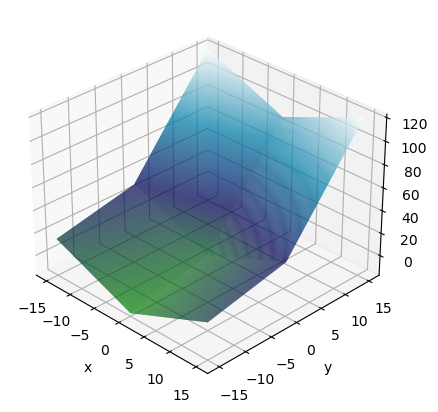
\includegraphics[width=8cm]{figures/sublinear_output.png}
\end{center}

\begin{itembox}[l]{\underline{Definition (Positively Homogeneous and Subadditive) }}
  A function $f$ is \textbf{positively homogeneous} if this $f$ satisfies the condition

  \begin{equation}
    f(\lambda x) = \lambda f(x),\:for \:all\: x \in{\mathbb{E}},\: \lambda \in{\mathbb{R}}_+. \notag
  \end{equation}

  Also a function $f$ is \textbf{subadditive} if this $f$ satisfies the condition

  \begin{equation}
    f( x + y) \leq f(x) + f(y),\:for \:all\: x, y \in{\mathbb{E}}. \notag
  \end{equation}
\end{itembox}

\begin{itembox}[l]{\underline{Proposition }}
  If a proper function $f$
  is sublinear then $-f(x) \leq f(-x)$ for all $x$ in $\mathbb{E}$.
\end{itembox}

\begin{proof}
  We show that it holds $-f(x) \leq f(-x)$ for all $x$ in $\mathbb{E}$.

  By the assumption of sublinear of $f$, we can use the inequality

  \begin{equation}
    f(\lambda x + \mu y) \leq \lambda f(x) + \mu f(y),\:for \:all\: x, y \in{\mathbb{E}},\: \lambda, \mu \in{\mathbb{R}}_+. \notag
  \end{equation}

  For any $x$ and $y$, we take $y=-x$ since ${\mathbb{E}}$ is a vector space, and also take $\lambda=\mu=1$. These values and the above assumption, we get the inequality

  \begin{equation}
    f(x + (-x)) \leq f(x) + f(-x). \notag
  \end{equation}

  By $f(0) = 0$,

  $\because$ Since $f$ is proper, $\exists x_0 \in \mathbb{E} \:s.t.\: f(x_0) < +\infty$. Then $f(0) = f(0 \cdot x) = 0 \cdot f(x) = 0$


  \begin{equation}
    0 \leq f(x) + f(-x). \notag
  \end{equation}

  Therefore we got $-f(x) \leq f(-x)$ for all $x$ in $\mathbb{E}$.
\end{proof}

\begin{itembox}[l]{\underline{Proposition (the former of Proposition 3.1.1) }}
  If the function $f$ is sublinear if and only if $f$ is positively homogeneous and subadditive.
\end{itembox}

\begin{proof}
  We show that

  \begin{center}
    $f$ is sublinear $\Leftrightarrow$ f is positively homogeneous and subadditive.
  \end{center}

  ($\Rightarrow$) By the definition of sublinear of $f$, for any $y$ we take $y=0$ and $\mu=0$. Then f is positively homogeneous. Like that, the subadditive of $f$ holds; you should put $\lambda=\mu=1$ to the inequality of sublinear.

  ($\Leftarrow$) By the definition of subadditive and positively homogeneous of $f$, $\forall x, y \in{\mathbb{E}},\: \lambda, \mu \in{\mathbb{R}}_+$,

  \begin{equation}
    f(\lambda x + \mu y) \leq f(\lambda x) + f(\mu y) = \lambda f(x) + \mu f(y) . \notag
  \end{equation}

  Therefore we completed to prove it.
\end{proof}

\begin{itembox}[l]{\underline{Definition (Lineality Space) }}
  The $lineality\:space$ of a
  sublinear function $f$, denoted by lin$f$, is the set

  \begin{equation}
      \text{lin} f = \{x \in \mathbb{E}\:|\:-f(x) = f(-x)\}. \notag
  \end{equation}
\end{itembox}

\begin{center}
  \fbox{
    \begin{minipage}{.8\textwidth}
      The following result (whose proof is left as an exercise) shows this set is a subspace.
    \end{minipage}
    }
\end{center}

\begin{itembox}[l]{\underline{Proposition 3.1.1 (Sublinearity) }}
  A function $f$ : $\mathbb{E}$ $\to$ $ \left ( -\infty ,+\infty \right ] $ is sublinear if and only if it is positively homogeneous and subadditive. For a sublinear function $f$, the lineality space lin$f$ is the largest subspace of $\mathbb{E}$ on
which $f$ is linear.
\end{itembox}

\begin{proof}
  The former proposition has already been proved. Accordingly we show the latter one, that the way of proof is two steps;

  \begin{enumerate}[label=\Roman*,align=CenterWithParen]
    \item lin$f$ is a subspace of $\mathbb{E}$.
    \item lin$f$ is the ``largest'' subspace of $\mathbb{E}$.
  \end{enumerate}

  ( $\mathrm{I}$ ) We show that

  \begin{enumerate}[label=\roman*,align=CenterWithParen]
    \item $\forall x, y \in \text{lin} f$, $x + y \in \text{lin} f$.
    \item $\forall x \in \text{lin} f$, $\alpha \in{\mathbb{R}}$, $\alpha x \in \text{lin} f$ .
  \end{enumerate}

  ( $\mathrm{i}$ ) We prove that $\forall x, y \in \text{lin}f$,

  \begin{center}
    $-f(x+y) = f(-x-y)$.
  \end{center}

  For any $x$ and $y$, by the definition of linearity space, it holds that

  \begin{center}
    $-f(x) = f(-x)$ and
    $-f(y) = f(-y)$.
  \end{center}

  And, Since f is sublinear, we have $f(x + y) \leq f(x) + f(y)$. Using the result of the above proposition about a sublinear property, we can get the inequality:

  \begin{center}
    $-f(x+y) \geq - f(x) - f(y) = f(-x) + f(-y) \geq f(-x-y) = f(-(x+y)) \geq -f(x+y)$.
  \end{center}

  This inequality means that $-f(x+y) = f(-x-y)$.

  ( $\mathrm{ii}$ ) We show that $\forall x \in \text{lin}f$, $\alpha \in{\mathbb{R}}$,

  \begin{center}
    $-f(\alpha x) = f(-\alpha x)$.
  \end{center}

  By the definition of positively homogeneous of $f$ and the definition of lineality space,

  \begin{center}
    $-f(\alpha x) = - \alpha f(x) = \alpha f(-x) = f(- \alpha x)$.
  \end{center}

  For the result of ( $\mathrm{i}$ ) and ( $\mathrm{ii}$ ), $\text{lin}f$ is a subspace of $\mathbb{E}$.

  ( $\mathrm{II}$ ) We show that for a sublinear function $f$ it holds that

  \begin{center}
    $\forall V \subset \mathbb{E}$, where $V$ is subspace of $\mathbb{E}$, $V \subset \text{lin}f$
  \end{center}

  For any $x$ in $V$, $-x \in V$ holds because $V$ is a subspace of $\mathbb{E}$. Since $f$ is linear,

  \begin{center}
    $0 = f(0) = f(x + (-x)) = f(x) + f(-x)$.
  \end{center}

  Therefore $\text{lin}f$ is the largest subspace of $\mathbb{E}$.
\end{proof}

\begin{center}
  \fbox{
    \begin{minipage}{.8\textwidth}
      As in the First order sufficient condition (2.1.2), it is easy to check that if the point $\bar{x}$ lies in the domain of the convex function $f$ then the directional derivative $f'(\bar{x};\cdot)$ is well-defined and positively homogeneous, taking values in $ \left [ -\infty ,+\infty \right ] $. The core of a set $C$ (written $\text{core} (C)$) is the set of points $x$ in $C$ such that for any direction $d$ in $\mathbb{E}$, $x + td$ lies in $C$ for all small real $t$. This set clearly contains the interior of $C$, although it may be larger (Exercise 2).
    \end{minipage}
  }
\end{center}

\begin{itembox}[l]{\underline{Definition (the core of a set) }}
  Let $C \subset \mathbb{E}$. The $\textbf{core}$ of the set $C$ is defined as

  \begin{center}
    $\text{core} (C)$ $\coloneqq$ $\{x \in \mathbb{E} \:|\: \forall d \in \mathbb{E}, \exists t_0 > 0 \:s.t.\: \forall t (0<t<t_0), x+td \in C \}$ .
  \end{center}
\end{itembox}


\begin{itembox}[l]{\underline{Exercise 2 (Core versus interior) }}
  Considering the set in $\mathbb{R}^2$

  \begin{center}
    $D=\{(x,y) \:|\: y = 0 \:or\: |y| \geq x^2 \}$ .
  \end{center}

  Prove $0 \in \text{core} (D) \backslash \text{int} (D) $
\end{itembox}

Figure($\text{core} (D)$):



\begin{center}
  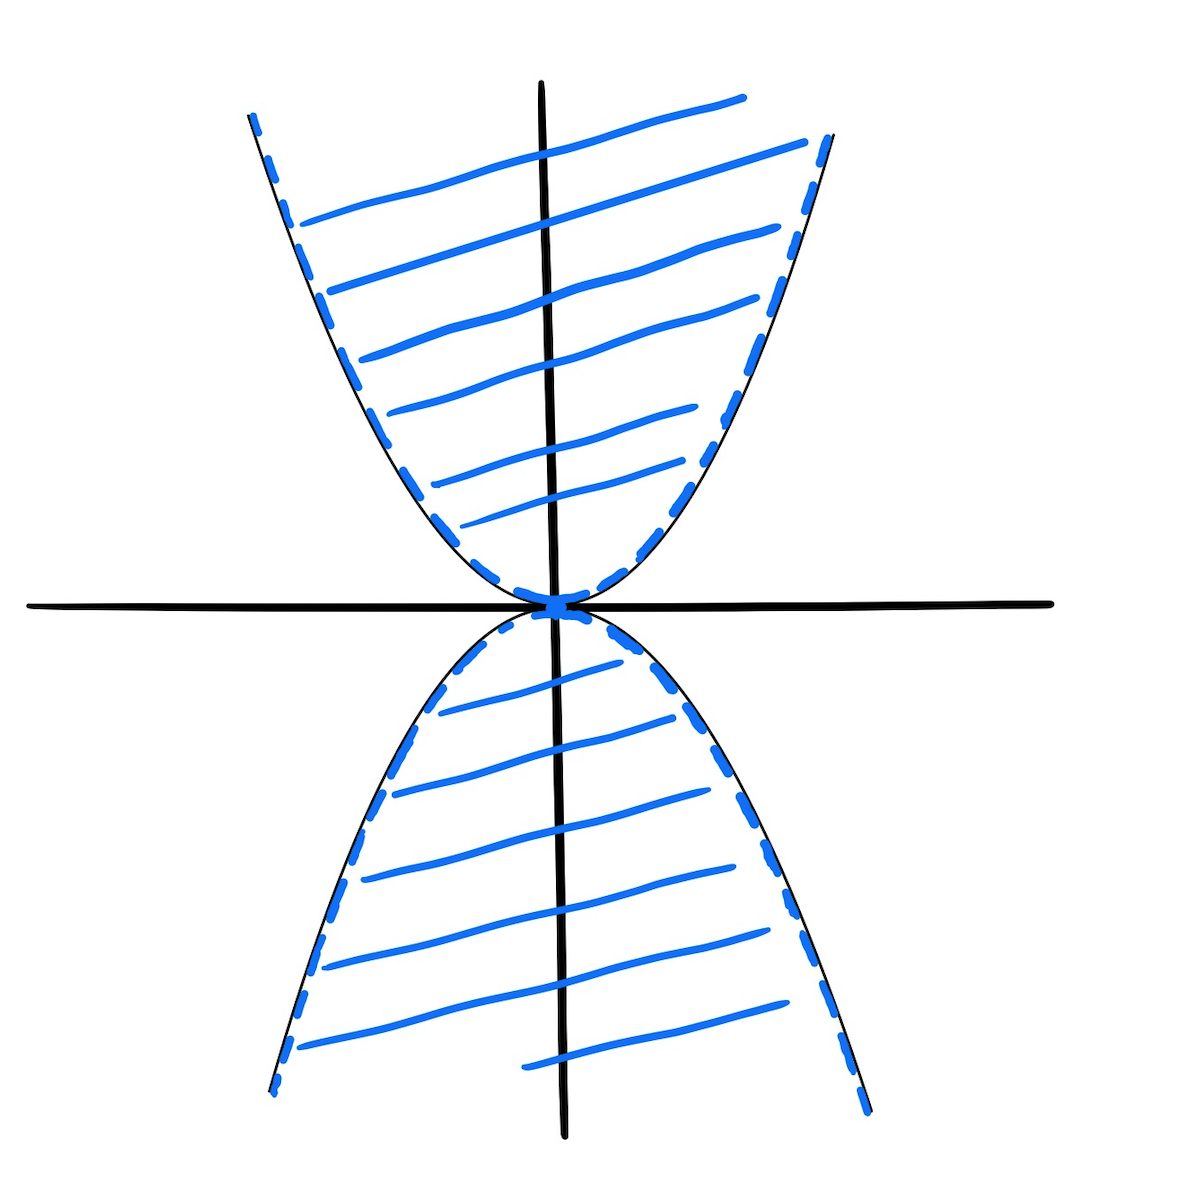
\includegraphics[width=8cm]{figures/core_versus_interior.png}
\end{center}

\begin{itembox}[l]{\underline{Proposition 3.1.2 (Sublinearity of the directional derivative) }}
  If the function $f$ : $\mathbb{E}$ $\to$ $ \left ( -\infty ,+\infty \right ] $ is convex then for any points $\bar{x}$ in $\text{core}(\text{dom} f)$, the directional derivative $f'(\bar{x};\cdot)$ is everywhere finite and sublinear.
\end{itembox}

\begin{proof}
  For $d$ in $\mathbb{E}$ and nonzero $t$ in $\mathbb{R}$, define

  \begin{equation}
    g(d;t) = \frac{f(\bar{x}+td) - f(\bar{x})}{t}. \notag
  \end{equation}

  By convexity we deduce, for $0<t\leq s \in \mathbb{R}$, the inequality

  \begin{equation}
    g(d;-s) \leq g(d;-t) \leq g(d;t) \leq g(d;s). \notag
  \end{equation}

  $\because$ $\forall t_1,t_2 (0 < t_1 \leq t_2)$, $\mathop{\underline{g(d;t_1) \leq g(d;t_2)}}\limits_{(1)}$, $\mathop{\underline{g(d;-t_2) \leq g(d;-t_1)}}\limits_{(2)}$, and $\mathop{\underline{g(d;-t_1) \leq g(d;t_1)}}\limits_{(3)}$.

  (1) We use the convexity of $f$.

  (2) It's leaded from (1) $\times (-1)$.

  (3) We can get since $f(\bar{x})$ is the middle points of $f(\bar{x}+td)$ and $f(\bar{x}-td)$.

  Since $\bar{x}$ lies in $\text{core($\text{dom}f$)}$, for small $s > 0$ both $g(d;-s)$ and $g(d;s)$ are finite, so as $t\downarrow 0$ we have

  \begin{equation}
    +\infty > g(d;s) \geq g(d;t) \downarrow f'(\bar{x};d) \geq g(d; -s) > -\infty. \notag
  \end{equation}

  Again by convexity we have, for any directions $d$ and $e$ in $\mathbb{E}$ and real $t>0$,

  \begin{equation}
    g(d+e;t) \leq g(d;2t) + g(e;2t). \notag
  \end{equation}

  $\because$

  \begin{equation}
    \begin{split}
      g(d+e;t) &= \frac{f(\bar{x}+t(d+e))-f(\bar{x})}{t}\\
      &= \frac{2f(\bar{x}+2t(\frac{1}{2}d+\frac{1}{2}e))-2f(\bar{x})}{2t}\\
      &= \frac{2f(\frac{1}{2}(\bar{x}+2td)+\frac{1}{2}(\bar{x}+2te))-2f(\bar{x})}{2t}\\
      &\leq \frac{f(\bar{x}+2td)-f(\bar{x})}{2t} + \frac{f(\bar{x}+2te)-f(\bar{x})}{2t}\\
      &= g(d;2t) + g(e;2t) \notag
    \end{split}
  \end{equation}

  Now letting $t \downarrow 0$ gives subadditivity of $f'(\bar{x};\cdot)$. The positively homogeneity is easy to check.

  $\because$ If $\lambda=0$, it's clear. $\forall d \in \mathbb{E},\lambda > 0, t>0$,

  \begin{equation}
    \begin{split}
      g(\lambda d;t) &= \frac{f(\bar{x}+t\lambda d) - f(\bar{x})}{t}\\
      &= \frac{\lambda (f(\bar{x}+t\lambda d) - f(\bar{x}))}{\lambda t}\\
      &= \lambda g(d;\lambda t) \notag
    \end{split}
  \end{equation}
\end{proof}

\begin{center}
  \fbox{
    \begin{minipage}{.8\textwidth}
      The idea of the derivative is fundamental in analysis because it allows us to approximate a wide class of functions using $\textit{linear functions}$. In optimization we are concerned specifically with the minimization of functions,

      and hence often a $\textit{one-sided approximation}$ is sufficient. In place of the gradient we therefore consider $\textit{subgradients}$, those elements $\phi$ of $\mathbb{E}$ satisfying

      \begin{equation}
        \left\langle \phi ,x-\bar{x}\right\rangle \leq f(x) - f(\bar{x})\:\text{for all points $x \in \mathbb{E}$} \tag*{(3.1.4)}
      \end{equation}

      We denote the set of subgradients (called the $\textit{subdifferential}$) by $\partial f(\bar{x})$, defining $\partial f(\bar{x})= \emptyset $ for  $\bar{x}$ not in $\text{dom}f$. The subdifferential is always a closed convex set. We can think of $\partial f(\bar{x})$ as the value at  $\bar{x}$ of the ``multifunction'' or ``set-valued map'' $\partial f$ : $\mathbb{E}$ $\to$ $\mathbb{E}$. The importance of such maps is another of our themes. We define its $\textit{domain}$

      \begin{equation}
        \text{dom} \partial f= \{ x\in\mathbb{E} \:|\: \partial f(x) \ne \emptyset \} \notag
      \end{equation}

      (Exercise 19). We say $f$ is $\textit{essentially strictly convex}$ if it is strictly convex on any convex subset of $\text{dom}\partial f$.

      The following very easy observation suggests the fundamental significance of subgradients in optimization.
    \end{minipage}
  }
\end{center}

\begin{itembox}[l]{\underline{Definition (Subgradient and Subdifferential) }}
  Let $f$ : $\mathbb{E}$ $\to$ $ \left ( -\infty ,+\infty \right ] $ and $\bar{x}$ in $\mathbb{E}$. If it holds that

  \begin{equation}
    \exists \phi \in \mathbb{E} \:s.t.\: f(x) \geq f(\bar{x}) + \left\langle \phi, x-\bar{x} \right\rangle, \forall x \in \mathbb{E} \notag
  \end{equation}

  then $\phi$ is called the subgradient of $f$ at $\bar{x}$.

  Also, the set of all subgradients of $f$ at $\bar{x}$ is called the subdifferential of $f$ at $\bar{x}$, denoted by $\partial f(\bar{x})$, that is

  \begin{equation}
    \partial f(\bar{x}) \coloneqq \{\phi \in \mathbb{E}\:|\:f(x) \geq f(\bar{x}) + \left\langle \phi, x-\bar{x} \right\rangle, \forall x \in \mathbb{E} \}. \notag
  \end{equation}
\end{itembox}

Observation(1):

We consider the inequality as the relation between two functions. The  graph is written as the shifted one of $y=\left\langle \phi,x \right\rangle$ with the direction of $(x_0,f(x_0))$.

\begin{equation}
  \begin{split}
    y &= f(x) \\
    y &= \left\langle \phi,x \right\rangle + f(x_0) \notag
  \end{split}
\end{equation}

Figure:

\begin{center}
  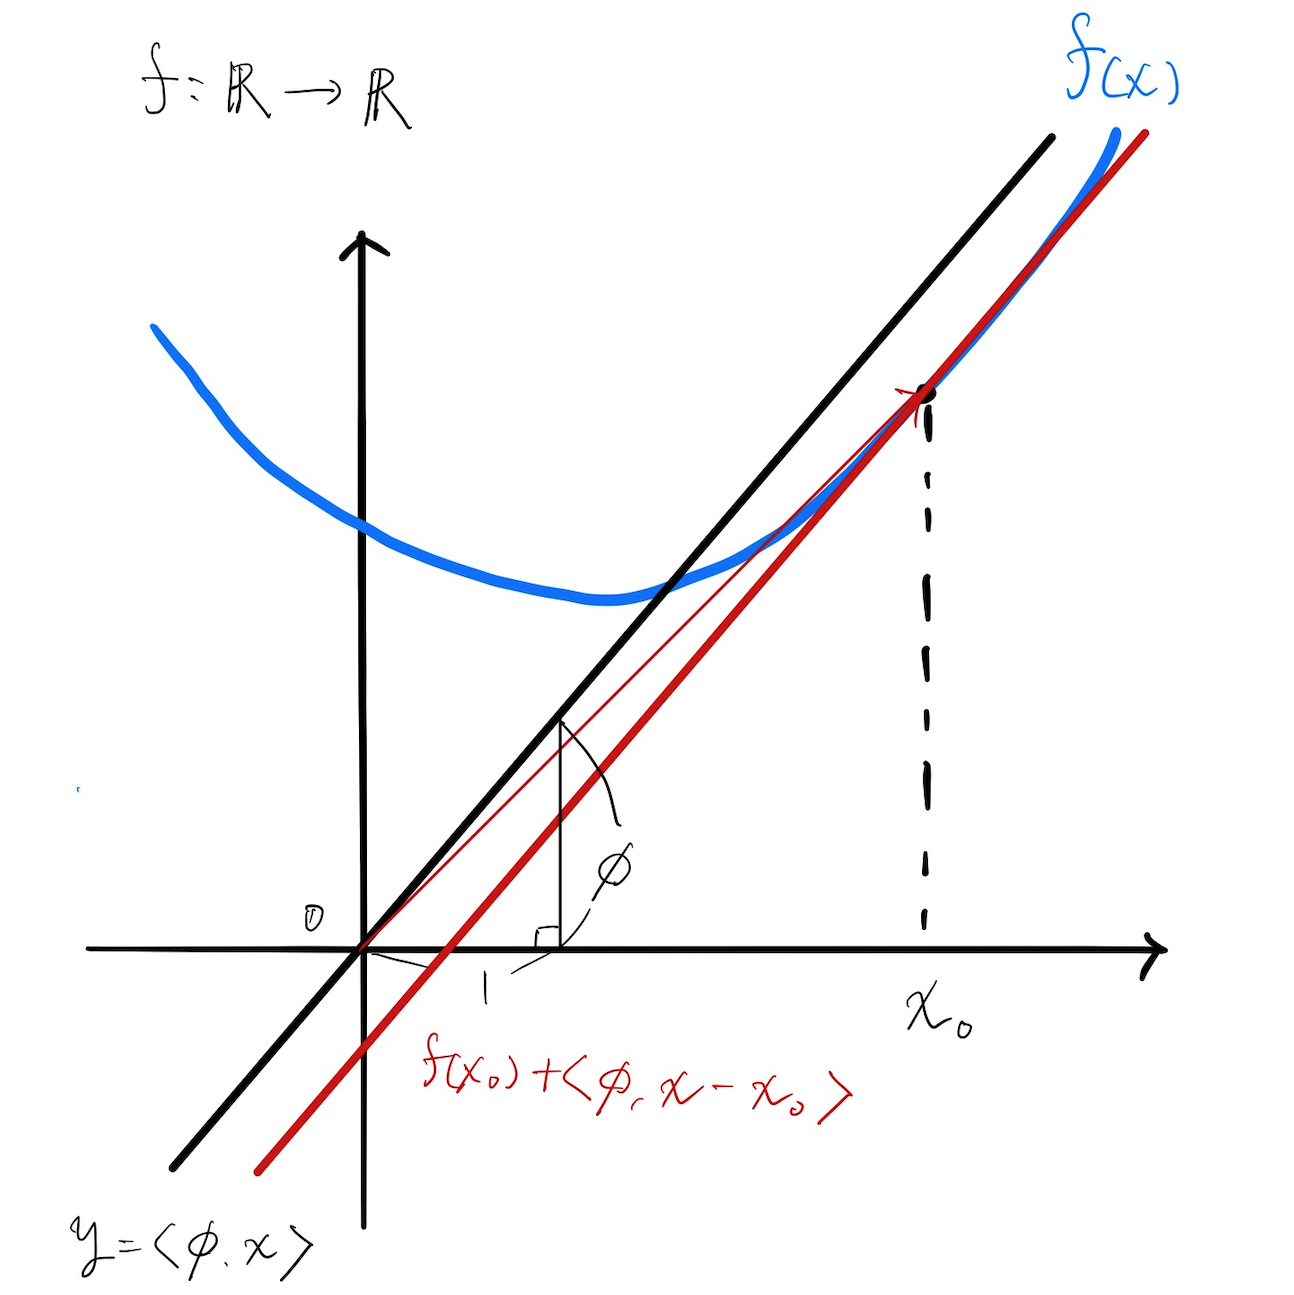
\includegraphics[width=8cm]{figures/subgradient_(1).png}
\end{center}

Observation(2):

We consider the inequality as the inner product.

\begin{equation}
  \begin{split}
    f(x) \geq f(\bar{x}) + \left\langle \phi, x-\bar{x} \right\rangle\\
    \left\langle \phi, x-\bar{x} \right\rangle + f(\bar{x}) - f(x)\leq 0\\
    \left\langle \phi, x-\bar{x} \right\rangle + (-1)(f(x) - f(\bar{x}))\leq 0\\
    \left\langle \binom{\phi}{-1},\binom{x}{f(x)} - \binom{x_0}{f(x_0)} \right\rangle \leq 0 \notag
  \end{split}
\end{equation}

Figure:

\begin{center}
  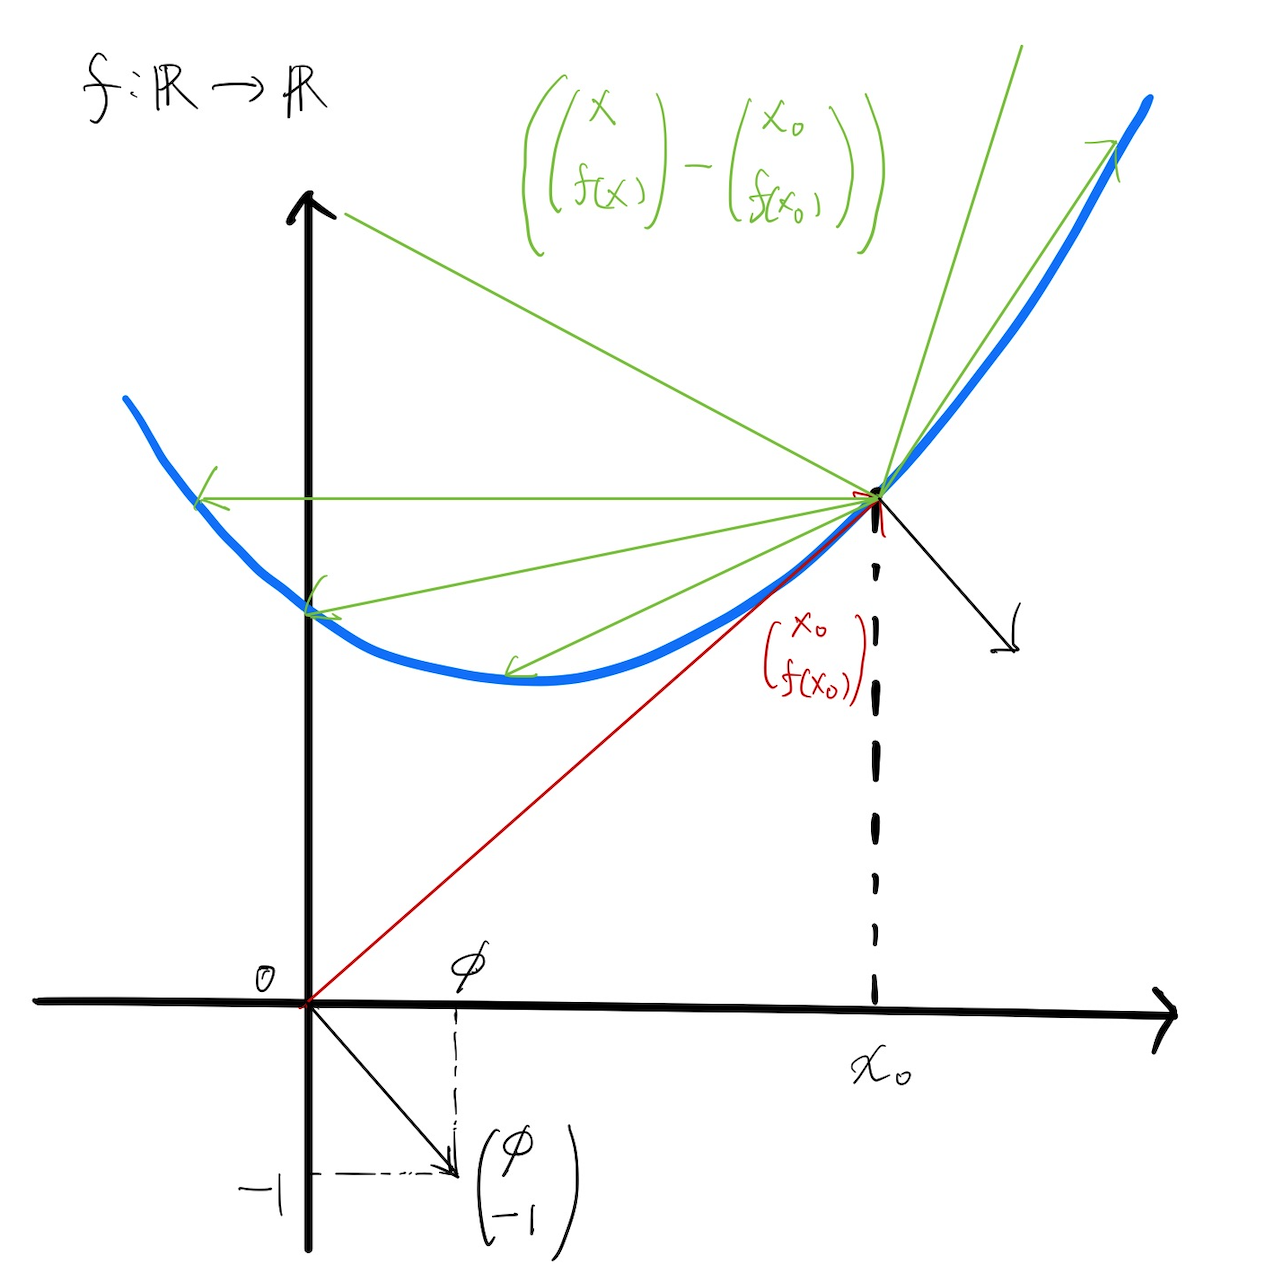
\includegraphics[width=8cm]{figures/subgradient_(2).png}
\end{center}

\begin{itembox}[l]{\underline{Exercise 19 (Domain of subdifferential) }}
  If the function $f$ : $\mathbb{R}^2$ $\to$ $ \left ( -\infty ,+\infty \right ] $ is defined by

  \begin{equation}
    f(x_1,x_2) =
    \begin{cases}
      \text{max}\{1-\sqrt{x_1}, |x_2|  \} & \text{if}\:x_1 \geq 0, \\
      +\infty & \text{otherwise}. \notag
    \end{cases}
  \end{equation}

  prove that $f$ is convex but that $\text{dom}\partial f$ is not convex.
\end{itembox}

Figure:

\begin{center}
  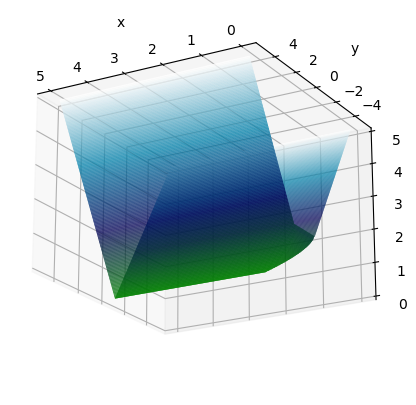
\includegraphics[width=7cm]{figures/subgradients_at_optimality.png}
\end{center}

\begin{itembox}[l]{\underline{Proposition 3.1.5 (Subgradients at optimality) }}
  For any proper functions $f$ : $\mathbb{E}$ $\to$ $ \left ( -\infty ,+\infty \right ] $, the points $\bar{x}$ is a (global) minimizer of $f$ if and only if the condition $0 \in \partial f(\bar{x})$ holds.
\end{itembox}

\begin{proof}
  The definition that $\bar{x} \in \mathbb{E}$ is a global minimizer of $f$ is

  \begin{equation}
    \forall x \in \mathbb{E},f(\bar{x}) \leq f(x).
  \end{equation}

  Also $0 \in \partial f$ means that

  \begin{equation}
    \forall x \in \mathbb{E}, f(x) \geq f(\bar{x}) + \left\langle 0, x-\bar{x} \right\rangle.
  \end{equation}

  We prove (1) $\Rightarrow $ (2) and  (1) $\Leftarrow $ (2).

  ($\Rightarrow$) Paying attention to the property of proper of $f$, $\forall x \in \mathbb{E}$

  \begin{equation}
    \begin{split}
      f(\bar{x}) \leq f(x)\\
      0 \leq f(x) - f(\bar{x})\\
      \left\langle 0, x-\bar{x} \right\rangle \leq f(x) - f(\bar{x}). \notag
    \end{split}
  \end{equation}

  It means that $0 \in \partial f(\bar{x})$ holds.

  ($\Leftarrow$) By (2), like above, $\forall x \in \mathbb{E}$

  \begin{equation}
    \begin{split}
      \left\langle 0, x-\bar{x} \right\rangle \leq f(x) - f(\bar{x})\\
      0 \leq f(x) - f(\bar{x})\\
      f(\bar{x}) \leq f(x). \notag
    \end{split}
  \end{equation}

  That is, $\bar{x}$ is a global minimizer of $f$.

  Therefore we have got (1) $\Leftrightarrow$ (2).

\end{proof}

\begin{center}
  \fbox{
    \begin{minipage}{.8\textwidth}
      Alternatively put, minimizers of $f$ correspond exactly to ``zeroes'' of $\partial f$.
      The derivative is a local property whereas the subgradient definition (3.1.4) describes a global property. The main result of this section shows
      that the set of subgradients of a convex function is usually \textit{nonempty}, and
      that we can describe it locally in terms of the directional derivative. We
      begin with another simple exercise.
    \end{minipage}
  }
\end{center}

\begin{itembox}[l]{\underline{Proposition 3.1.6 (Subgradients and directional derivatives) }}
  If the function $f$ : $\mathbb{E}$ $\to$ $ \left ( -\infty ,+\infty \right ] $ is convex and the point $\bar{x}$ lies in $\text{dom}f$, then an element $\phi$ of $\mathbb{E}$ is a subgradient of $f$ at $\bar{x}$ if and only if it satisfies $\left\langle \phi,\cdot \right\rangle \leq f'(\bar{x};\cdot)$.
\end{itembox}

  \begin{enumerate}[label=\arabic*,align=CenterWithParen]
    \item $\phi$ is a subgradient of $f$ at $\bar{x}$.
    \item $\forall d \in \mathbb{E}, \left\langle \phi,d \right\rangle \leq f'(\bar{x};d)$.
  \end{enumerate}

\begin{proof}

  We show (1) $\Rightarrow$ (2) and (1) $\Leftarrow$ (2).

  ($\Rightarrow$)

  ($\Leftarrow$)

\end{proof}

\begin{center}
  \fbox{
    \begin{minipage}{.8\textwidth}
      The idea behind the construction of a subgradient for a function $f$ that we present here is rather simple. recursively construct a decreasing sequence of sublinear functions which, after translation, minorize $f$. At each step we guarantee one extra direction of linearity. The basic step is summarized in the following exercise.
    \end{minipage}
  }
\end{center}

\begin{itembox}[l]{\underline{Lemma 3.1.7 }}
  Suppose that the function $p$ : $\mathbb{E}$ $\to$ $ \left ( -\infty ,+\infty \right ] $ is sublinear and that the points $\bar{x}$ lies in $\text{core}(\text{dom }p)$. Then the function $q(\cdot) = p'(\bar{x};\cdot)$ satisfies the conditions

  \begin{enumerate}[label=\roman*,align=CenterWithParen]
    \item $q(\lambda \bar{x}) = \lambda p (\bar{x})$ for all real $\lambda$,
    \item $q \leq p$, and
    \item $\text{lin}q \supset \text{lin}p + \text{span}\{\bar{x}\}$.
  \end{enumerate}
\end{itembox}

\begin{proof} We show these relations.

  ( $\mathrm{i}$ ) Since $\bar{x} \in \text{core}(\text{dom}p)$, for a given $\lambda$

  \begin{equation}
    \exists\hat{t}>0 \:s.t.\: \forall t \in (0,\hat{t}), \bar{x}+t(\lambda \bar{x}) \in \text{dom}p \:\text{and}\: \bar{x}+t(-\lambda \bar{x}) \in \text{dom}p. \tag*{(1)}
  \end{equation}

  Also given $\lambda \in \mathbb{R}$, it holds that

  \begin{equation}
    \exists\widetilde{t}>0 \:s.t.\: \forall t \in (-\widetilde{t},\widetilde{t}), 1+\lambda t>0 \:\text{and}\: 1-\lambda t<0. \tag*{(2)}
  \end{equation}


  For the $t$ which satisfies (1) and (2), i.e., for $t = \text{min}\{\hat{t},\widetilde{t}\} >0$,

  \begin{equation}
    \begin{split}
      q(\lambda \bar{x}) = p'(\bar{x};\lambda \bar{x}) &= \lim_{t \downarrow 0} \frac{p(\bar{x}+\lambda \bar{x}t)-p(\bar{x})}{t} \\
      &= \lim_{t \downarrow 0} \frac{p((1 + \lambda t)\bar{x}) - p(\bar{x})}{t} \\
      &= \lim_{t \downarrow 0} \frac{(1 + \lambda t)p(\bar{x}) - p(\bar{x})}{t} \because \text{$f$ is sublinear}\\
      &= \lambda p(\bar{x}). \notag
    \end{split}
  \end{equation}

  ( $\mathrm{ii}$ )$\forall x \in \mathbb{E}$, there exist $t>0$ satisfying (1) that is described with not $\bar{x}$ but $x$,

  \begin{equation}
    \begin{split}
      q(x) = p'(\bar{x};x) &= \lim_{t \downarrow 0} \frac{p(\bar{x}+tx)-p(\bar{x})}{t} \\
      &\leq \lim_{t \downarrow 0} \frac{p(\bar{x}) + tp(x) - p(\bar{x})}{t} \because \text{$f$ is sublinear}\\
      &= p(x). \notag
    \end{split}
  \end{equation}

  ( $\mathrm{iii}$ ) We show that

  \begin{equation}
    \forall y \in \text{lin}\:p + \text{span}\{\bar{x}\}, y \in \text{lin}\:q. \notag
  \end{equation}

  Since $q$ is sublinear, it holds that $-q(y) \leq q(-y)$. Accordingly we prove the reverse, $-q(y) \geq q(-y)$.

  As $y \in \text{lin}\:p + \text{span}\{\bar{x}\}$,

  \begin{equation}
    \exists x \in \text{lin}\:p, \alpha \in \mathbb{R} \:s.t.\: y=x+\alpha \bar{x}. \notag
  \end{equation}

  Also since x is in $\text{lin}\:p$, $-p(x)=p(-x)$ holds by the definition of lineality space.

  Then,

  \begin{equation}
    \begin{split}
      q(-y) &= q(-(x+\alpha \bar{x}))\\
      &\leq q(-x) + q(-\alpha \bar{x}) \because \text{$q$ is sublinear}\\
      &\leq p(-x) + -p(\alpha \bar{x}) \because \text{Lemma3.1.7 ( $\mathrm{i}$ ), ( $\mathrm{ii}$ )}\\
      &= -p(x) + -p(\alpha \bar{x}) \because \text{$x \in \text{lin}\:p$}\\
      &\leq -q(x) - q(\alpha \bar{x}) \because \text{Lemma3.1.7 ( $\mathrm{ii}$ )}\\
      &= (-1)(q(x)+q(\alpha \bar{x}))\\
      &= (-1)(q(x+\alpha \bar{x}))\\
      &= -q(y). \notag
    \end{split}
  \end{equation}

  Therefore it holds that $\text{lin}q \supset \text{lin}p + \text{span}\{\bar{x}\}$.

\end{proof}

\begin{center}
  \fbox{
    \begin{minipage}{.8\textwidth}
      With this tool we are now ready for the main result, which gives conditions guaranteeing the existence of a subgradient. Proposition 3.1.6 showed how to identify subgradients from directional derivatives; this next result shows how to move in the reverse direction.
    \end{minipage}
  }
\end{center}

\begin{itembox}[l]{\underline{Theorem 3.1.8 (Max formula) }}
  If the function $f$ : $\mathbb{E}$ $\to$ $ \left ( -\infty ,+\infty \right ] $ is convex then any points $\bar{x}$ in $\text{core}(\text{dom}f)$ and any direction $d$ $\in \mathbb{E}$ satisfying

  \begin{equation}
    f'(\bar{x};d) = \text{max}\{\left\langle \phi , d\right\rangle \:|\: \phi \in \partial f(\bar{x})\} \tag*{(3.1.9)}
  \end{equation}

  In particular, the subdifferential $\partial f(\bar{x})$ is nonempty.
\end{itembox}

\begin{proof}
  In view of Proposition 3.1.6 we simply have to show that for  any fixed $d$ in $\mathbb{E}$ there is a subgradient $\phi$ satisfying $\left\langle \phi , d\right\rangle = f'(\bar{x};d)$. Choose a bases $\{e_1,e_2,\dots,e_n\}$ for $\mathbb{E}$ with $e_1=d$ if $d$ is nonzero. Now define a sequence of functions $p_0,p_1,\dots,p_n$ recursively by $p_0(\cdot)=f'(\bar{x};\cdot)$, and $p_k(\cdot)=p_{k-1}'(e_k;\cdot)$ for $k=1,2,\dots,n$. We essentially show that $p_n(\cdot)$ is the required subgradient.


\end{proof}

\end{document}
